\section{Genetic Programming}
\label{sec:genetic_programming}
  \emph{Genetic Programming} (GP)~\autocite{kozaGeneticProgrammingProgramming1992a,kozaGeneticProgrammingII1994,poliFieldGuideGenetic2008a,yuIntroductionEvolutionaryAlgorithms2010}
  is a specialized branch of Evolutionary Algorithms (EA) which focuses on 
  evolving a population of computer programs to solve a given problem.
  One can perceive GP as an extension of Genetic Algorithms (GA), the key
  distinction being the problem each approach solves: GA optimizes parameters to 
  enhance a given function, whilst GP induces programs.\footnote{%
      For a formal definition of program induction, refer to 
      \vref{def:program_induction}.
  }

  Despite these differences, GP and GA share various characteristics such as the 
  utilization of a population of individuals, the employment of a fitness function
  to evaluate the individuals, and the application of genetic operators to 
  generate new individuals.
  Notwithstanding, GP adopts a unique representation for the individuals and 
  unique genetic operators.

  \begin{remark}
    Although GP operates a fitness-guided search in the space of computer 
    programs, it can be deemed as an optimization problem, akin to GA.
  \end{remark}

  Each individual in a GP population embodies a computer program composed of a set
  of primitives, referred to as \emph{functions} and \emph{terminals}.
  An intuitive way to comprehend primitives is by visualizing a composite pattern
  where the functions equate to composite objects and the terminals to leaf
  objects (refer to \vref{fig:composite_pattern}).
  An \emph{abstract syntax tree} (AST) is an example of a program representation
  where the functions correspond to the internal nodes, and the terminals to the
  leaf nodes.

  \begin{figure}[ht!]
    \centering
    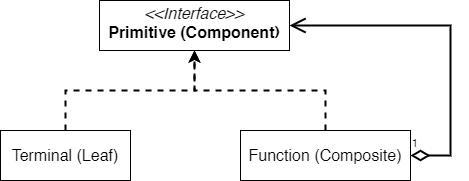
\includegraphics[width=0.4\textwidth]{img/theoretical_framework/GP Composite.png}
    \caption{
      The composite structure of a GP individual, illustrating the relationship
      between functions and terminals
    }
    \label{fig:composite_pattern}
  \end{figure}

  The general GP algorithm is represented in \vref{alg:genetic_programming}, which
  closely resembles the GA algorithm with the main disparity being the nature of
  the \textit{genetic operators} in GP.

  \begin{algorithm}[ht!]
    \begin{algorithmic}[1]
      \State Generate an initial population by recursively building random programs.
      \State Execute each program and assign a fitness value to it.
      \Repeat
        \State \(\mathit{parents} \gets \mathrm{selectParents}(\mathit{population})\) 
          \Comment{Parent selection for reproduction}
        \State \(\mathrm{alter}(\mathit{offspring})\) 
          \Comment{Apply genetic operators to offspring}
        \State \(\mathit{population} \gets \mathrm{selectSurvivors}(
          \mathit{population}, \mathit{offspring})\) 
          \Comment{Survivor selection to form next generation}
      \Until{termination condition is met} 
        \Comment{
          Termination can be a fixed number of generations, or a satisfactory 
          fitness level, etc.
        }
      \State \textbf{return} \(\mathrm{fittest}(\mathit{population})\) 
        \Comment{Return the best solution found}
    \end{algorithmic}
    \caption{
      Outline of the Genetic Programming algorithm, showcasing its structural 
      similarities with the Genetic Algorithm
    }
    \label{alg:genetic_programming}
  \end{algorithm}

  In the ensuing sections, we will delve into the fundamental components of a GP
  algorithm and elucidate them through an example.

  \subimport{./}{Representation.tex}
  \subimport{./}{Initialization.tex}
%